\documentclass[mathserif,serif]{beamer}

\usepackage[utf8]{inputenc}
\usepackage{graphicx}
\usecolortheme{beaver}
\graphicspath{{./images/}}


\title{Traditional Approaches to Machine Learning}
\subtitle{A brief overview of different classic Machine Learning Algorithms}

\author{Tilman Roeder}
\date{\today}


\begin{document}

\begin{frame}
  \maketitle
\end{frame}

\begin{frame}
  \frametitle{Today}
  \tableofcontents
\end{frame}

\section{Naive Bayes Classifiers}
\frame{\sectionpage}

\begin{frame}
  \frametitle{(Super Brief) Primer in Bayesian Statistic}

  Define conditional probabilities
  \begin{equation}
    P(X|Y) P(Y) = P(X \cap Y)
  \end{equation}
  \pause

  Which immediately gives Bayes Theorem
  \begin{equation}
    P(X|Y) = \frac{P(Y|X) P(X)}{P(Y)} = \frac{P(Y|X) P(X)}{\sum_X P(Y|X) P(X)}
  \end{equation}
  \pause

  In Bayesian Statistics probabilities quantify our `degree of believe'.

  Bayes Theorem allows us to `update' our believes (prior) based on new
  evidence (data) to obtain a new believe (posterior).
\end{frame}

\begin{frame}
  \frametitle{Naive Bayes Classifiers}
  \begin{itemize}
    \item<1-> Given a set of possible labels $\{X_i\}$ and an observation $Y \in \{Y_i\}$
    \item<2-> We seek $P(X|Y)$
    \item<3-> Apply Bayes Theorem to compute posterior probability
    \item<4-> Conditional probabilities are based on simple (naive) heuristics
  \end{itemize}
\end{frame}

\begin{frame}
  \frametitle{Example: Spam Filtering}
  Given a message $M$ consisting of words $(W_1, W_2, \dots, W_n)$, and assuming words occurrences
  are independent we have:
  \begin{equation}
    P(S|W) = \frac{P(W|S)P(S)}{P(W)} = \frac{P(S)\prod_i P(W_i|S)}{\sum_{s \in \{S, \neg S\}} P(s) \prod_i P(W_i|s)},
  \end{equation}
  where $P(S)$ is the probability of the message being spam.
\end{frame}

\begin{frame}
  \frametitle{Example: Spam Filtering}
  Note that the previous expression is prone to numeric instability. We can fix this by computing
  the probabilities in $log$ space:
  \begin{equation}
  \begin{split}
    \ln\left( \frac{1}{P(S|W)} - 1 \right) = \sum_i \ln\left( P(W_i|\neg S) \right) - \ln\left( P(W_i|S) \right) \\
      + \ln(P(\neg S)) - \ln(P(S))
  \end{split}
  \end{equation}
\end{frame}

\begin{frame}
  \frametitle{Example: Spam Filtering}
  What are $P(W|S)$, $P(W)$, and $P(S)$? \pause This is where we invent heuristics:
  \begin{itemize}
    \item $P(W|S) = $ fraction of spam words that are $W$
    \item $P(W|\neg S) = $ fraction of ham words that are $W$
    \item $P(S) = $ fraction of spam received in total (or unbiased: $\frac12$)
  \end{itemize}
  \pause
  These are very cheap to compute, and one of the oldest spam filters. Bayesian Classifiers are not
  as good as more advanced techniques. But for applications where speed and simplicity are important,
  they can be very competitive.
\end{frame}

\section{Support Vector Machines}
\frame{\sectionpage}

\begin{frame}
  \frametitle{Linear Separable Data}
  \begin{columns}
    \column{0.4\linewidth}
    \centering
    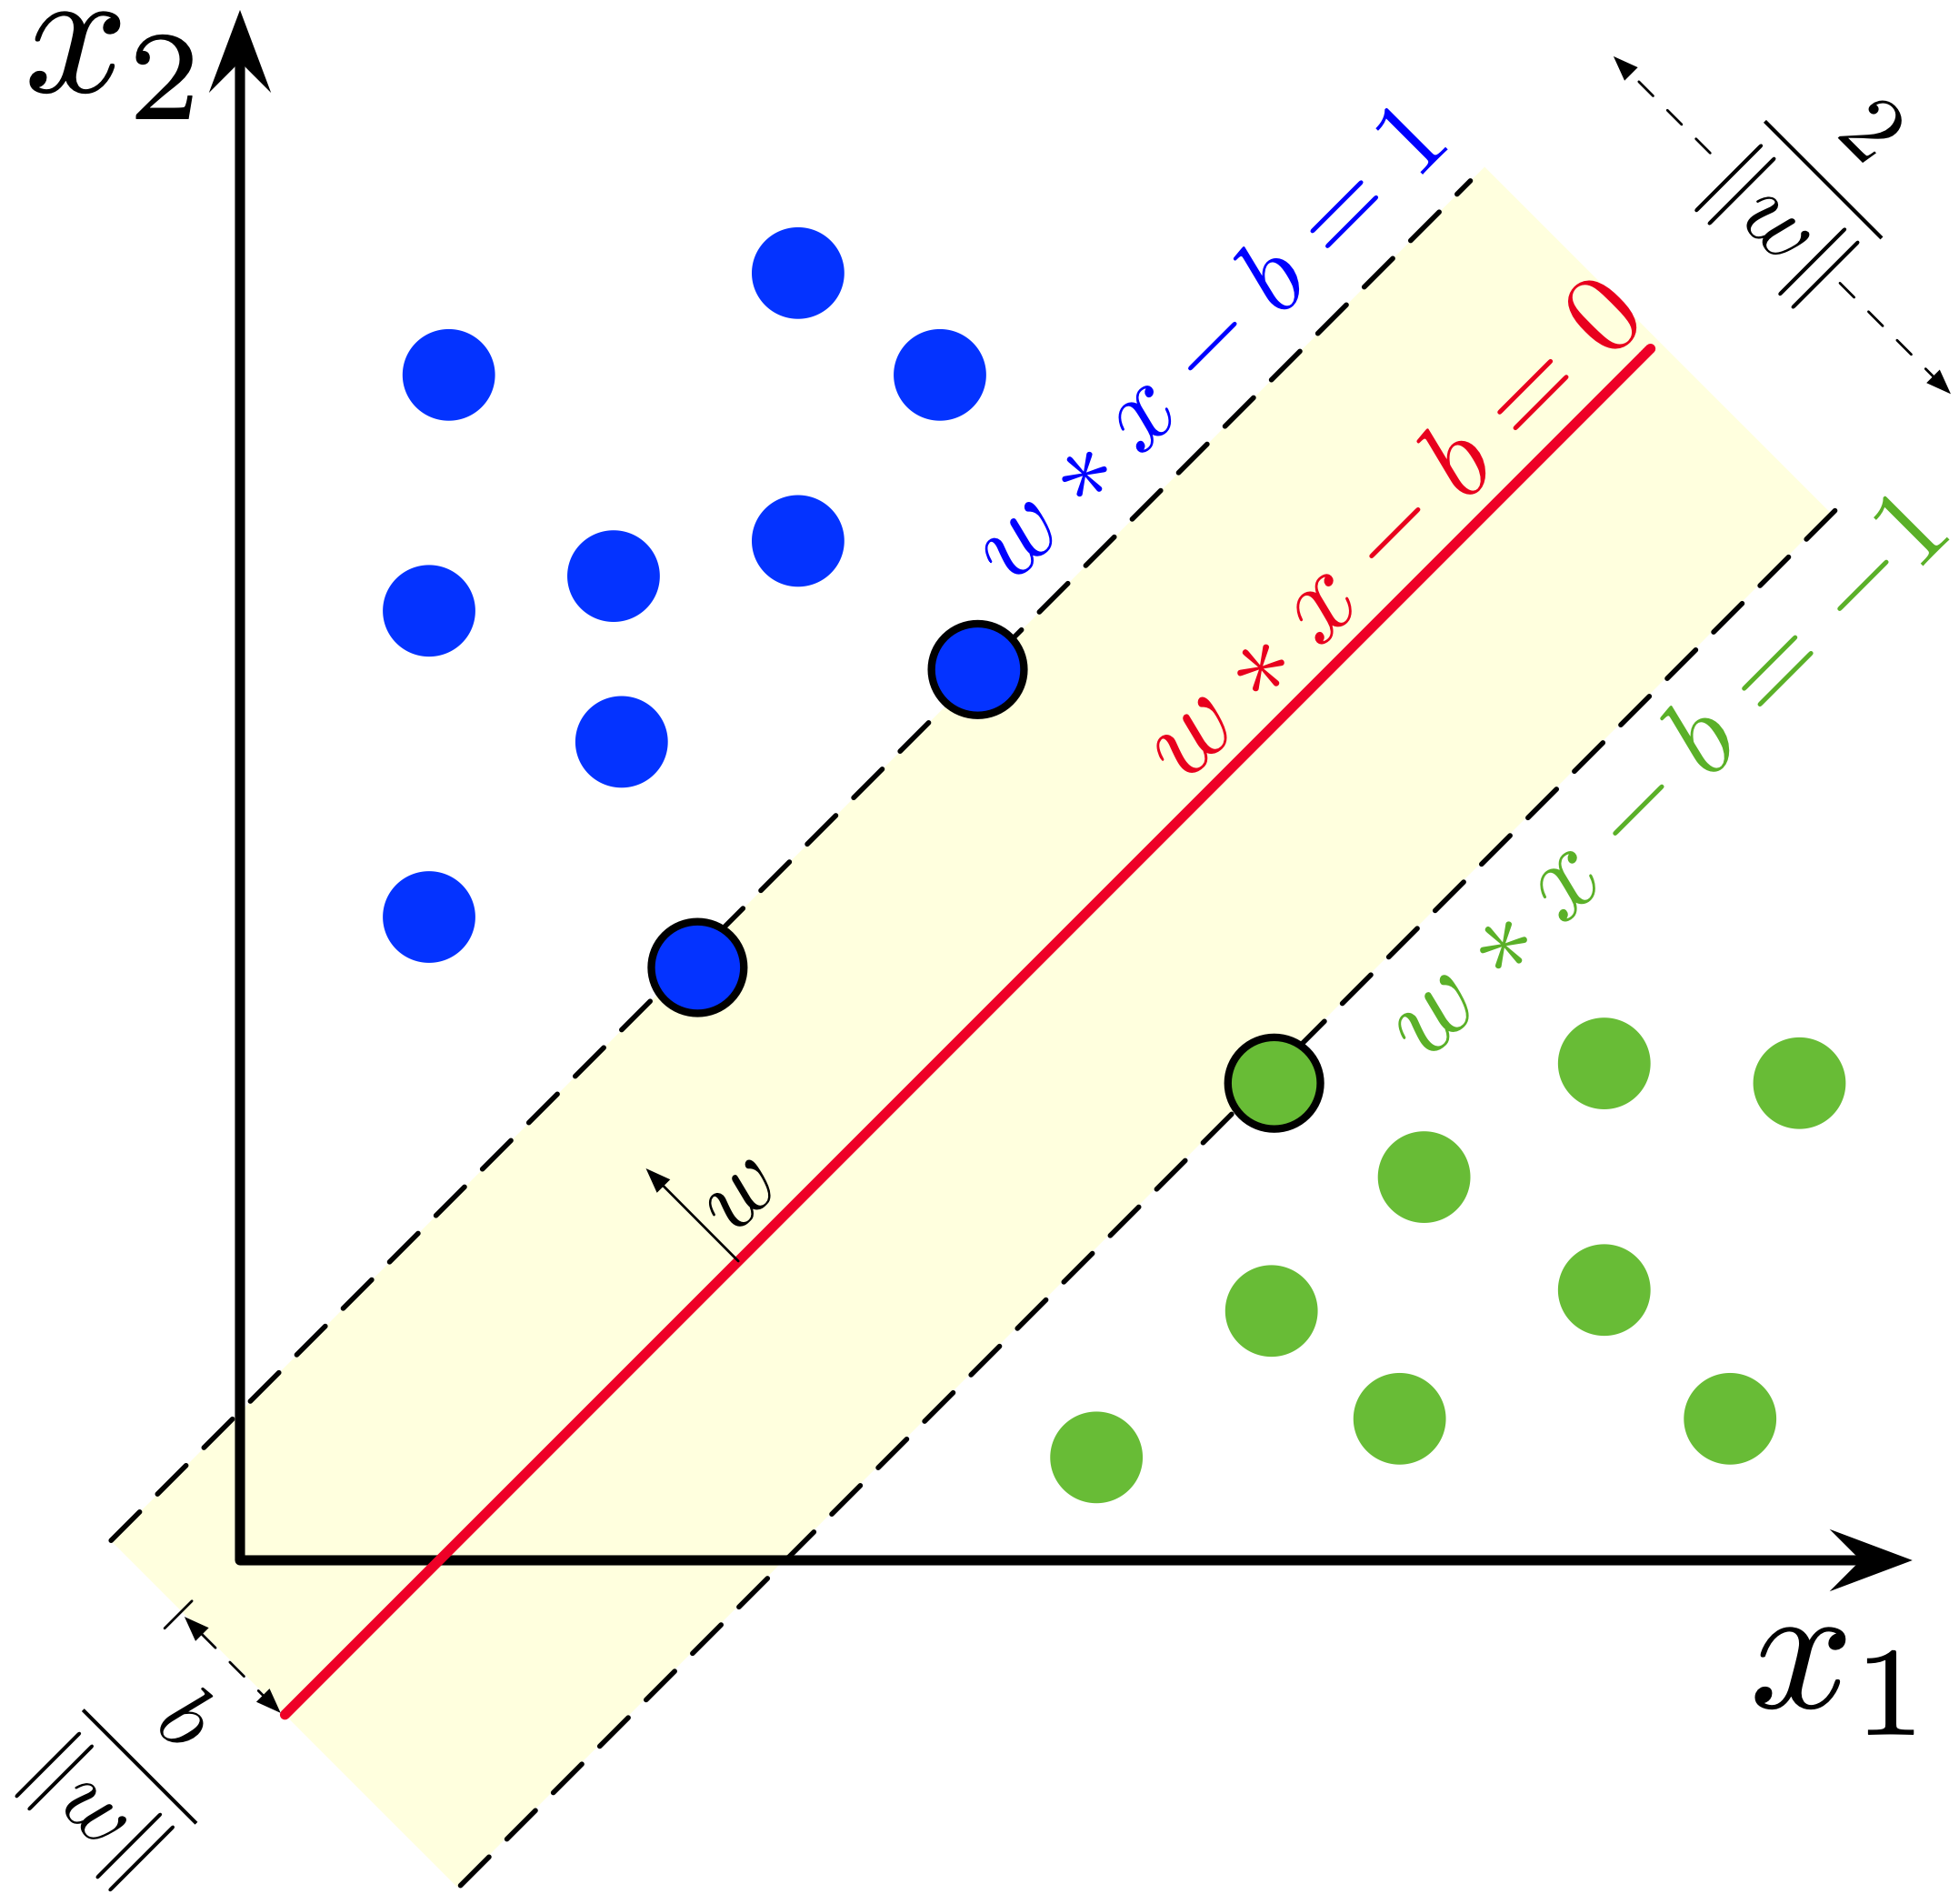
\includegraphics[width=5cm]{svm}
    \textit{\tiny(graphic by ZackWeinberg)}

    \column{0.6\linewidth}
    \begin{itemize}
      \item SVMs classify data with binary labels
      \item Classification is achieved by drawing a hyperplane between the data
    \end{itemize}
  \end{columns}
\end{frame}

\begin{frame}
  \frametitle{Support Vector Machine Classifier}
  A hyperplane $P$ in $\mathbb{R}^n$ is defined by
  \begin{equation}
    \vec{\omega} \cdot \vec{x} - b = 0,
  \end{equation}
  with $\vec{\omega}, \vec{x} \in \mathbb{R}^n$, $b \in \mathbb{R}$ and $\cdot$ denotes the inner product.

  \pause
  We can now define the Support Vector Machine classifier:
  \begin{equation}
    \tilde{y}(\vec{x}) = \operatorname{sign}(\vec{\omega} \cdot \vec{x} - b).
  \end{equation}

  \pause
  Note that the classifier has $n+1$ free parameters.
\end{frame}

\begin{frame}
  \frametitle{Hard Margin SVM}
  Consider a set of labeled points $\left\{ (\vec x_i, y_i) \right\}$, where
  $y_i \in \{-1, +1\}$.

  \pause
  Define two hyperplanes equidistant from $P$: $P_1$, $P_{-1}$ as
  \begin{equation}
    \vec{\omega} \cdot \vec{x} - b = \pm 1.
  \end{equation}
  Note that $P_{\pm1}$ have a distance of $\frac{2}{|\vec{\omega}|}$.

  \pause
  To find the SVM classifier we minimize $|\vec{\omega}|$, subject to the condition that
  $P$ correctly classifies the data:
  \begin{equation}
    y_i(\vec\omega \cdot \vec x_i - b) \geq 1
  \end{equation}

  \pause
  Notice that the parameters $\vec \omega, b$ are completely determined by those
  $\vec x_i$ which are closest to $P$. These are called the `support vectors'.
\end{frame}

\begin{frame}
  \frametitle{Soft Margin SVM}
  What happens when the data is not linearly separable?

  \pause
  We can use a soft-margin classifier instead. This is done by modifying the
  loss function:
  \begin{equation}
    L = \frac 1n \sum_i \max(0, 1 - y_i(\vec\omega \cdot \vec x_i - b)) + \lambda |\vec\omega|
  \end{equation}

  \pause
  We now find $\vec\omega, b$ by minimizing $L$.
\end{frame}

\begin{frame}
  \frametitle{The Kernel Trick}
  \begin{columns}
    \column{0.4\linewidth}
    \centering
    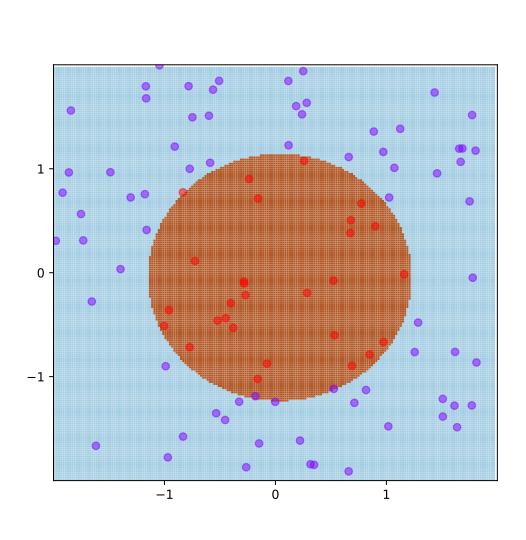
\includegraphics[width=5cm]{not_linear}
    \textit{\tiny(graphic by Shiyu Ji)}

    \column{0.6\linewidth}
    If the data is not linearly separable, a soft-margin SVM performs poorly.
  \end{columns}
\end{frame}

\begin{frame}
  \frametitle{The Kernel Trick}
  \begin{columns}
    \column{0.4\linewidth}
    \centering
    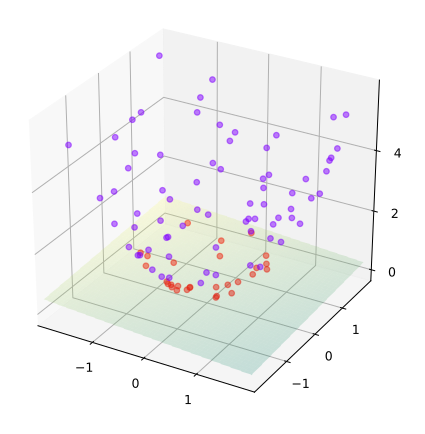
\includegraphics[width=5cm]{kernel_trick}
    \textit{\tiny(graphic by Shiyu Ji)}

    \column{0.6\linewidth}
    However, there may be a map $K: \mathbb{R}^n \to \mathbb{R}^m$ to a higher dimensional space
    $\mathbb{R}^{m>n}$, in which the data is linearly separable.
  \end{columns}
\end{frame}

\begin{frame}
  \frametitle{The Kernel Trick}
  Consider the case where (like in the picture) class $1$ lies inside the unit circle in $\mathbb{R}^2$.

  \pause
  Take the map
  \begin{equation}
    K(\vec x) = (x_1, x_2, x_1^2+x_2^2).
  \end{equation}

  \pause
  In this new space, the data is separated by the plane
  \begin{equation}
    \hat z \cdot \vec x - 1 = 0.
  \end{equation}

  \pause
  We further define $k: \mathbb{R}^2 \to \mathbb{R}$ such that
  \begin{equation}
    k(\vec x, \vec y) = K(\vec x) \cdot K(\vec y) = \vec x \cdot \vec y + |\vec x|^2 |\vec y|^2.
  \end{equation}

  \pause
  $k$ is called the `Kernel' and allows us to easily compute inner products, without having to
  explicitly map $\vec x_i$ to the higher dimensional space.

\end{frame}

\section{Decision Trees}
\frame{\sectionpage}

\end{document}
